\section{Problème de la recherche d'ordre}
La QPE peut être utilisée pour résoudre plusieurs problèmes dont le problème de la recherche d'ordre \cite{nielsen00}. Il consiste à trouver pour $a,N \in \mathbb{N}^*$ le plus petit entier $r \leq N$ (qu'on appelle l'ordre) tel que $a^r \equiv 1\text{ mod } N$ où $a < N$ et pgcd($a, N$) = 1. Pour résoudre ce problème avec la QPE, on emploie l'unitaire suivante : 

\begin{equation}
    U_a\ket*{x} = \ket*{ax \text{ mod } N}
\end{equation}

On ajoute aussi que $U_a$ agit seulement lorsque $0 \leq x < N$. Autrement, on considère qu'il s'agit de la matrice identité. On remarque par (6) que $U_a^r\ket*{x} = \ket*{a^r x \text{ mod } N} = \ket*{(a^r \text{ mod } N)(x \text{ mod } N)\text{ mod } N} = \ket*{(1\cdot x) \text{ mod } N} = \ket*{x}$, c'est-à-dire que $U_a^r = \mathbb{I}$. Ainsi, les valeurs propres $\lambda_s$ des vecteurs propres $\ket*{u_s}$ de $U_a$ sont de la forme $e^{2\pi i \frac{s}{r}}$ où $s$ est un certain entier, puisqu'il faut que $\lambda_s^r = 1$. De plus, on montre que les vecteurs propres $\ket*{u_s}$ de $U_a$ sont $\ket*{u_s} = \frac{1}{\sqrt{r}}\sum_{k=0}^{r-1}e^{-2\pi ik\frac{s}{r}}\ket*{a^k \text{ mod } N}$.
\begin{equation*}
    U_a\ket*{u_s} = \frac{1}{\sqrt{r}}\sum_{k=0}^{r-1}e^{-2\pi ik\frac{s}{r}}\ket*{a (a^{k} \text{ mod } N) \text{ mod } N} = \frac{1}{\sqrt{r}}\sum_{k=0}^{r-1}e^{-2\pi ik\frac{s}{r}}\ket*{(a \text{ mod } N) (a^{k} \text{ mod } N) \text{ mod } N}
\end{equation*}

\begin{equation*}
    = \frac{1}{\sqrt{r}}\sum_{k=0}^{r-1}e^{-2\pi ik\frac{s}{r}}\ket*{a^{k+1} \text{ mod } N} = \frac{1}{\sqrt{r}}\sum_{k^{'}=1}^{r}e^{-2\pi i(k^{'}-1)\frac{s}{r}}\ket*{a^{k^{'}}\text{ mod } N} = e^{2\pi i \frac{s}{r}} \frac{1}{\sqrt{r}}\sum_{k^{'}=1}^{r}e^{-2\pi ik^{'}\frac{s}{r}}\ket*{a^{k^{'}}\text{ mod } N}
\end{equation*}

\begin{equation*}
    = e^{2\pi i \frac{s}{r}}\frac{1}{\sqrt{r}}\sum_{k=0}^{r-1}e^{-2\pi ik\frac{s}{r}}\ket*{a^{k} \text{ mod } N} = e^{2\pi i \frac{s}{r}} \ket*{u_s}
\end{equation*}

Trouver l'ordre semble alors facile, car on aurait qu'à se servir de la QPE pour approximer $\frac{s}{r}$ et de là en tirer $r$. Mais avant de pouvoir utiliser la QPE, il faut s'assurer que $U_a$ soit unitaire et qu'un vecteur propre $\ket*{u_s}$ (ou qu'une superposition de ces vecteurs propres) peut facilement être préparé. 

On vérifie d'abord que $U_a$ est inversible. L'application de $U_a$ sur un état quelconque $\ket*{x}$ produit $\ket*{ax \text{ mod } N}$. On s'attend donc à ce que $U_a^{-1}$ effectue l'inverse multiplicatif modulo $N$ dont on a parlé à la section 1. Puisqu'on a comme condition initiale que pgcd($a, N$) = 1, on sait par la section 1 que $a^{-1}$ existe et donc que $U_a$ est inversible.  

\begin{equation*}
    U_a^{-1}\ket*{ax \text{ mod } N} = \ket*{a^{-1} (ax \text{ mod } N ) \text{ mod } N} = \ket*{(a^{-1}\text{ mod } N) (ax \text{ mod } N ) \text{ mod } N} = \ket*{(a^{-1}ax)\text{ mod } N}= \ket*{x}
\end{equation*}

Il reste maintenant à vérifier que $U_a^{-1} = U_a^{\dag}$, ce qui est équivalent à montrer que $U_a^{\dag}U_a = \mathbb{I}$. On calcule 

\begin{equation*}
    \bra*{x^{'}}U_a^{\dag}U_a\ket*{x} = \braket*{ax^{'} \text{ mod } N}{ax \text{ mod } N} = \delta_{x,x^{'}} \implies U_a^{\dag}U_a = \mathbb{I} \implies U_a^{\dag} = U_a^{-1}
\end{equation*}

et on voit bien que $U_a$ est unitaire.

À priori, préparer un état propre $\ket*{u_s}$ n'est pas évident, car selon sa définition, il faudrait connaître l'ordre $r$. Cependant, c'est exactement cette quantité qu'on cherche. Toutefois, on remarque que

\begin{equation*}
    \frac{1}{\sqrt{r}}\sum_{s=0}^{r-1}\ket*{u_s} = \frac{1}{\sqrt{r}} \sum_{k,s = 0}^{r-1}e^{-2\pi i k \frac{s}{r}}\ket*{a^k \text{ mod } N} = \sum_{k=0}^{r-1}\left(\frac{1}{r}\sum_{s=0}^{r-1}e^{-2\pi i k \frac{s}{r}}\right)\ket*{a^k \text{ mod } N}
\end{equation*}

Puis, on utilise la série géométrique 

\begin{equation*}
    \sum_{s=0}^{r-1}e^{-2\pi i k \frac{s}{r}} = \sum_{s=0}^{r-1}\left(e^{-2\pi i \frac{k}{r}}\right)^s = \frac{1 - e^{-2\pi ik}}{1 - e^{-2\pi i \frac{k}{r}}} = \delta_{k,0} \ 
\end{equation*}

pour en arriver à

\begin{equation*}
    \sum_{k=0}^{r-1}\delta_{k,0}\ket*{a^k \text{ mod } N} = \ket*{1}
\end{equation*}


Ainsi, l'état $\ket*{1}$ correspond à une certaine superposition de vecteurs propres de $U_a$ et permet une initialisation simple pour la QPE. Comme toutes les conditions sont remplies, la QPE sera capable d'obtenir une des valeurs propres $\frac{s}{r}$ d'un des états dans la superposition. À partir de là, on peut retrouver $r$ grâce aux fractions continues (section D du document complémentaire). Malgré tout, on ne sait absolument pas comment faire pour implémenter la transformation unitaire avec un circuit quantique. Les prochaines sections montreront les différents blocs nécessaires à sa construction.

\begin{figure}[H]
    \centering
    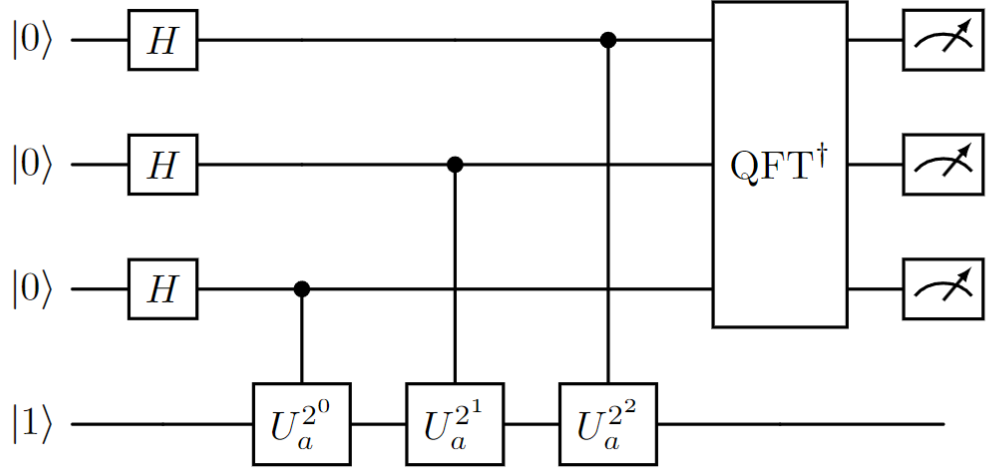
\includegraphics[scale=0.4]{images/circuit_ordre.png}
    \caption{Circuit du problème de la recherche d'ordre avec $m=3$}
\end{figure}